% \documentclass[../../diplom_data_assimilation.tex]{subfiles}
%use the following makro for all include paths (graphics, data files, other tex files,...)
% \makeatletter\@ifundefined{fromRoot}{\newcommand{\fromRoot}[1]{../../#1}}{}\makeatother
% \begin{document}
\chapter{Datenassimilation}
\section{Problemstellung}
Das Ziel der 4-D Datenassimilierung 
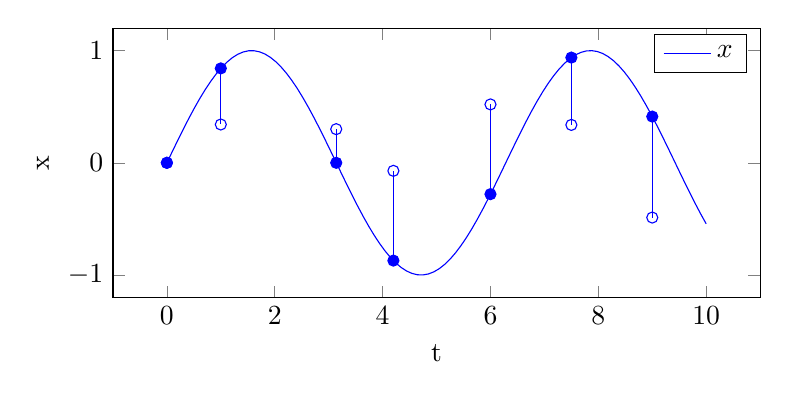
\begin{tikzpicture}
     \begin{axis}[width=9.8cm,height=5cm,xlabel=t,ylabel=x] 
     \addplot[blue,domain=0:10,samples=100]{sin(deg(x))};
     \addplot+[blue,draw=none,mark=*, mark options={blue},error bars/.cd, y dir=plus,y explicit,error mark=o,error mark options={blue,mark size=2pt}] 
     coordinates { 
      (0,0) +- (0,0) 
     (1,0.8415) +- (0.5,-0.5) 
     (3.14,0) +- (0.05,0.3) 
     (4.2,-0.8715) +- (0,0.8)
     (6.0,-0.27942) +- (0,0.8)
     (7.5,0.93799) +- (0.1,-0.6) 
     (9,0.41212) +- (0.3,-0.9)}; 
  \legend{$x$}
     \end{axis}
   \end{tikzpicture}

  
	
% \end{document}